\section{Custom Model Training and Evaluation}
\textbf{Owner: Peranavan.K -- 230474K}

Both custom CNNs were trained using the same split and training configuration: 20 epochs, batch size 32, Adam optimizer with learning rate 0.001, and sparse categorical crossentropy. The experiments were run in a CPU-only TensorFlow environment. Test-set evaluation reports accuracy, macro precision, macro recall, macro F1-score, and confusion matrices.

\begin{figure}[H]
\centering
\begin{subfigure}{0.48\linewidth}
\centering
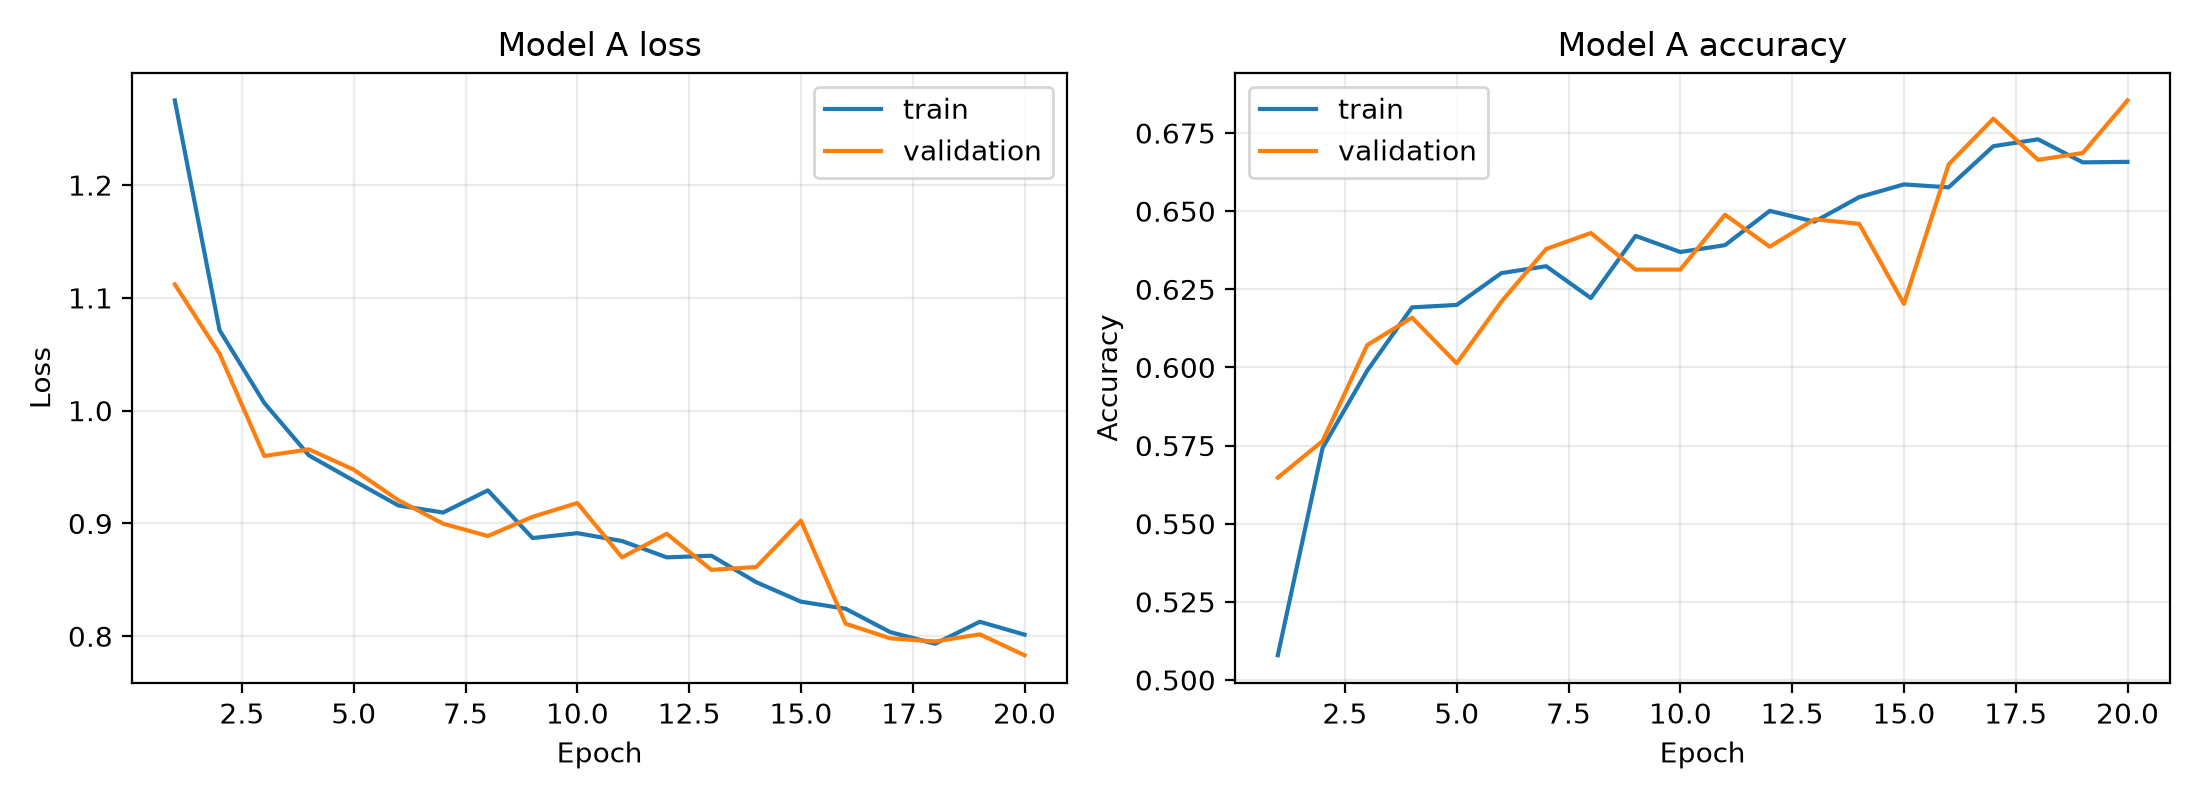
\includegraphics[width=\linewidth]{figures/model_a_history.png}
\caption{Model A learning curves.}
\label{fig:model_a_history}
\end{subfigure}
\hfill
\begin{subfigure}{0.48\linewidth}
\centering
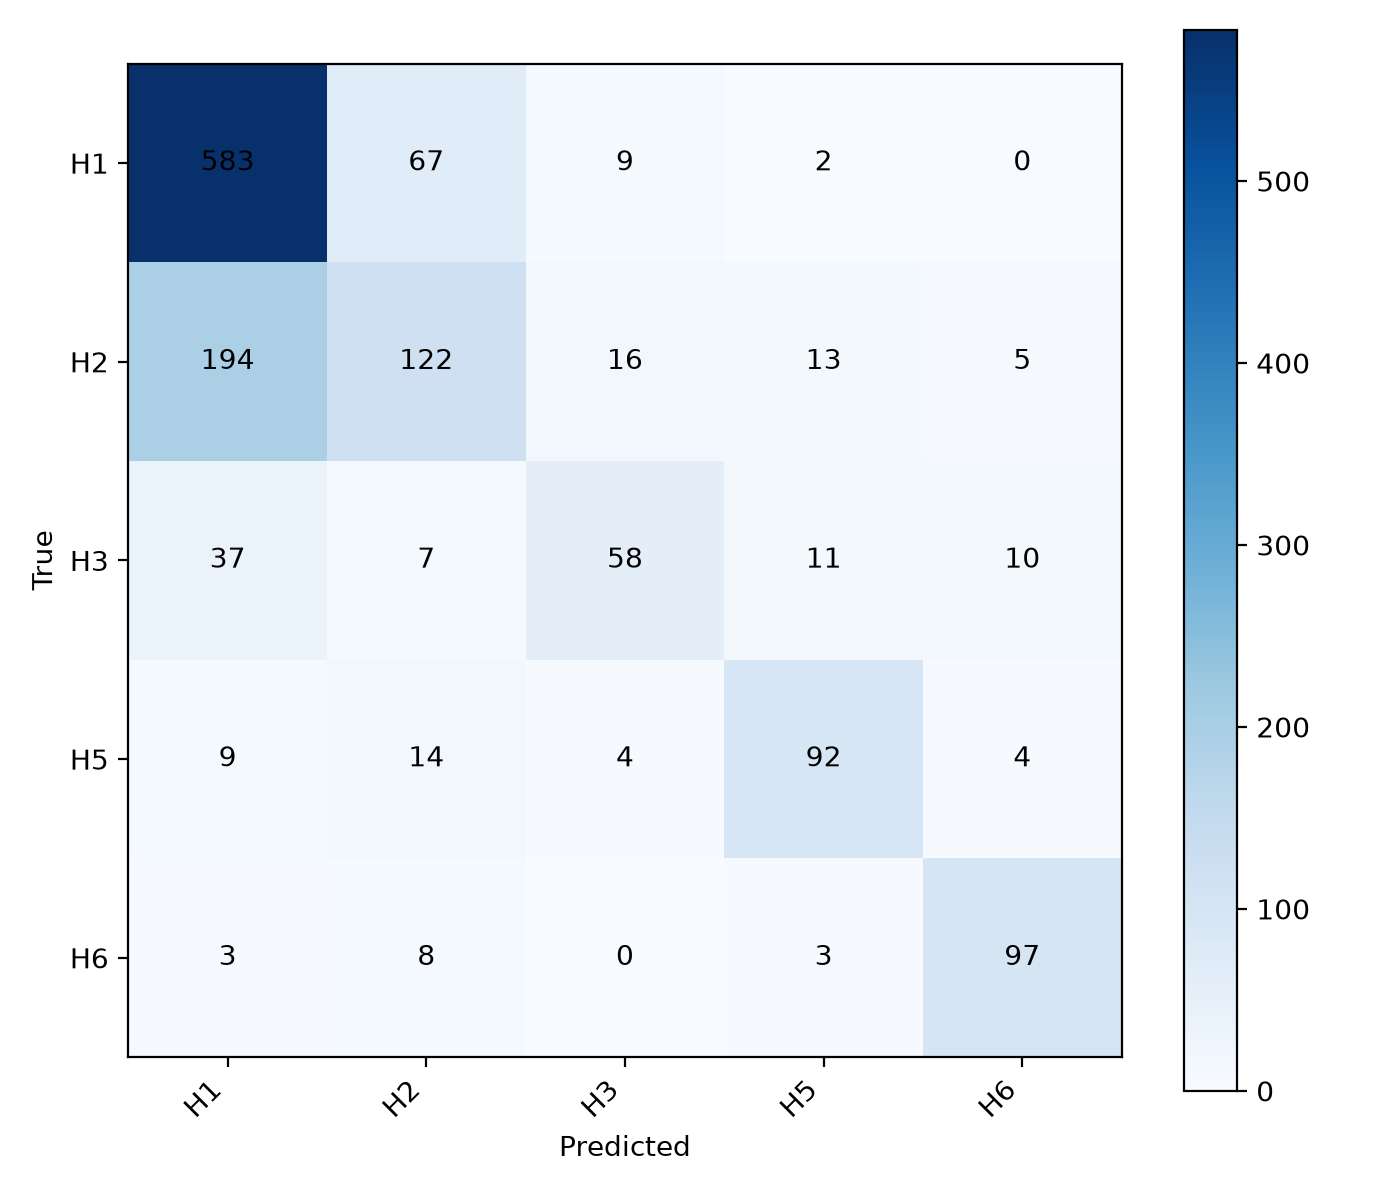
\includegraphics[width=\linewidth]{figures/model_a_confusion_matrix.png}
\caption{Model A confusion matrix.}
\label{fig:model_a_confusion}
\end{subfigure}
\caption{Model A training and test evaluation.}
\end{figure}

\begin{figure}[H]
\centering
\begin{subfigure}{0.48\linewidth}
\centering
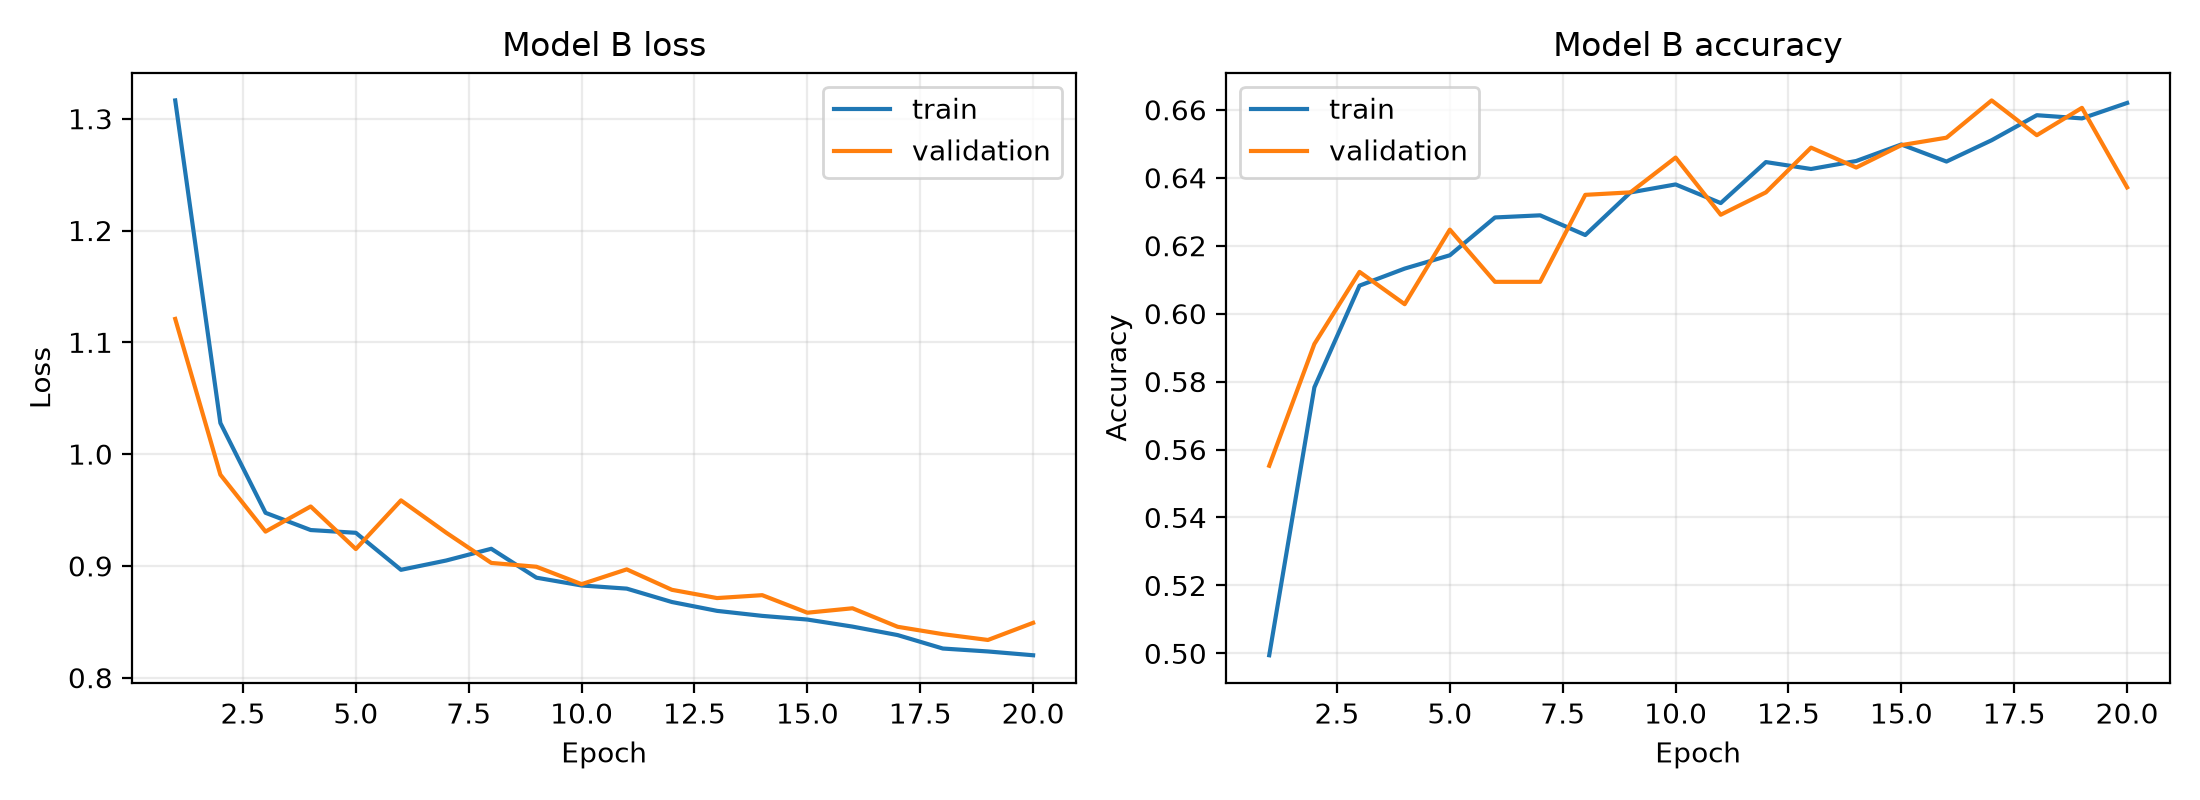
\includegraphics[width=\linewidth]{figures/model_b_history.png}
\caption{Model B learning curves.}
\label{fig:model_b_history}
\end{subfigure}
\hfill
\begin{subfigure}{0.48\linewidth}
\centering
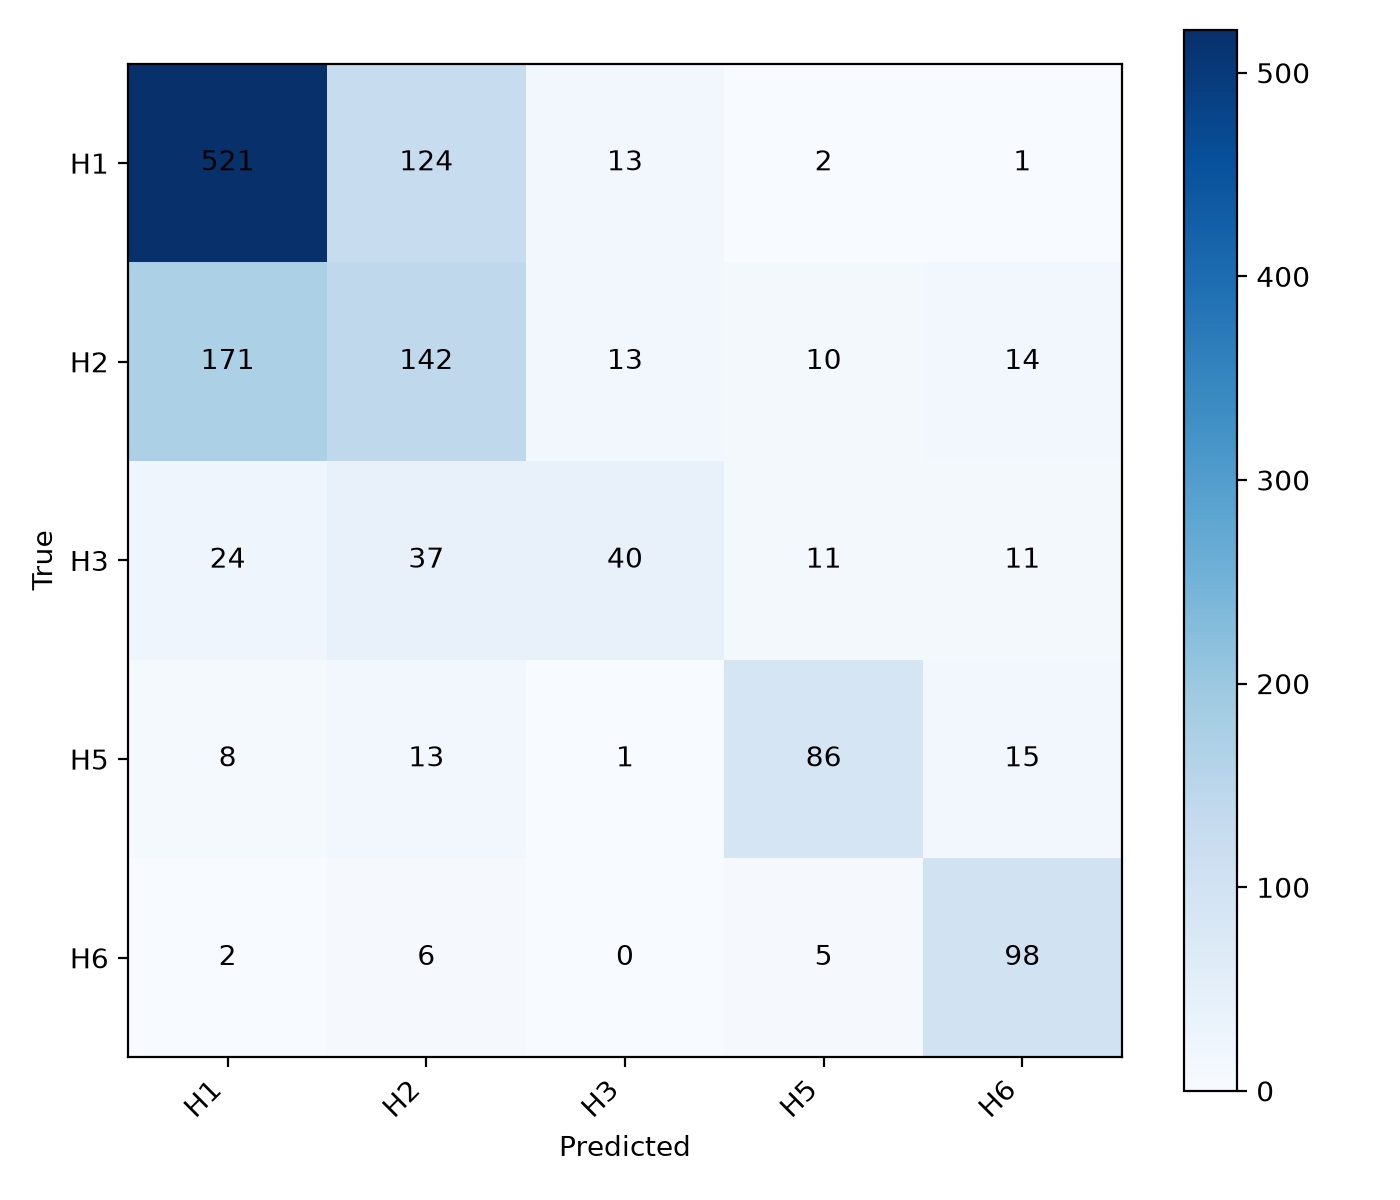
\includegraphics[width=\linewidth]{figures/model_b_confusion_matrix.png}
\caption{Model B confusion matrix.}
\label{fig:model_b_confusion}
\end{subfigure}
\caption{Model B training and test evaluation.}
\end{figure}

\begin{table}[H]
\centering
\caption{Custom CNN test-set comparison.}
\label{tab:custom_results}
\begin{tabular}{lrr}
\toprule
Metric & Model A & Model B \\
\midrule
Test accuracy & 0.6959 & 0.6484 \\
Macro precision & 0.7057 & 0.6430 \\
Macro recall & 0.6648 & 0.6202 \\
Macro F1-score & 0.6750 & 0.6209 \\
Parameters & 101,829 & 14,272 \\
FP32 parameter storage & 397.77 KB & 55.75 KB \\
Mean epoch time & 12.8958 s & 7.8730 s \\
\bottomrule
\end{tabular}
\end{table}

Model A gives higher classification performance, reaching 0.6959 test accuracy and 0.7057 macro precision. Model B trades away some accuracy for a much smaller footprint: it uses only 14,272 parameters and trains faster per epoch. This makes Model B the stronger candidate when memory and compute are the primary constraints.
